%%%%%%%%%%%%%%%%%%%%%%%%%%%%%%%%%%%%%%%%%
% Beamer Presentation
% LaTeX Template
% Version 1.0 (10/11/12)
%
% This template has been downloaded from:
% http://www.LaTeXTemplates.com
%
% License:
% CC BY-NC-SA 3.0 (http://creativecommons.org/licenses/by-nc-sa/3.0/)
%
%%%%%%%%%%%%%%%%%%%%%%%%%%%%%%%%%%%%%%%%%

%----------------------------------------------------------------------------------------
%	PACKAGES AND THEMES
%----------------------------------------------------------------------------------------

%\documentclass[UTF8,aspectratio=169,14pt]{ctexbeamer}
\documentclass[UTF8,aspectratio=169]{ctexbeamer}
\usepackage{hyperref}
\hypersetup{
	colorlinks=true,
	linkcolor=red,
	anchorcolor=blue,
	citecolor=green
}

\mode<presentation> {
	
	% The Beamer class comes with a number of default slide themes
	% which change the colors and layouts of slides. Below this is a list
	% of all the themes, uncomment each in turn to see what they look like.
	
	%\usetheme{default}
	%\usetheme{AnnArbor}
	%\usetheme{Antibes}
	%\usetheme{Bergen}
	%\usetheme{Berkeley}
	%\usetheme{Berlin}
	%\usetheme{Boadilla}
	%\usetheme{CambridgeUS}
	%\usetheme{Copenhagen}
	%\usetheme{Darmstadt}
	%\usetheme{Dresden}
	%\usetheme{Frankfurt}
	%\usetheme{Goettingen}
	%\usetheme{Hannover}
	%\usetheme{Ilmenau}
	%\usetheme{JuanLesPins}
	%\usetheme{Luebeck}
	\usetheme{Madrid}
	%\usetheme{Malmoe}
	%\usetheme{Marburg}
	%\usetheme{Montpellier}
	%\usetheme{PaloAlto}
	%\usetheme{Pittsburgh}
	%\usetheme{Rochester}
	%\usetheme{Singapore}
	%\usetheme{Szeged}
	%\usetheme{Warsaw}
	
	% As well as themes, the Beamer class has a number of color themes
	% for any slide theme. Uncomment each of these in turn to see how it
	% changes the colors of your current slide theme.
	
	%\usecolortheme{albatross}
	%\usecolortheme{beaver}
	%\usecolortheme{beetle}
	%\usecolortheme{crane}
	%\usecolortheme{dolphin}
	%\usecolortheme{dove}
	%\usecolortheme{fly}
	%\usecolortheme{lily}
	%\usecolortheme{orchid}
	%\usecolortheme{rose}
	%\usecolortheme{seagull}
	%\usecolortheme{seahorse}
	%\usecolortheme{whale}
	%\usecolortheme{wolverine}
	
	%\setbeamertemplate{footline} % To remove the footer line in all slides uncomment this line
	%\setbeamertemplate{footline}[page number] % To replace the footer line in all slides with a simple slide count uncomment this line
	
	%\setbeamertemplate{navigation symbols}{} % To remove the navigation symbols from the bottom of all slides uncomment this line
}

\usepackage{graphicx} % Allows including images
\graphicspath{{./figs/}}
\usepackage{booktabs} % Allows the use of \toprule, \midrule and \bottomrule in tables
\usepackage{longtable}
\usepackage{listings}
\usepackage{xcolor}
\lstset{numbers=left, %设置行号位置
	numberstyle=\tiny, %设置行号大小
	keywordstyle=\color{blue}, %设置关键字颜色
	commentstyle=\color[cmyk]{1,0,1,0}, %设置注释颜色
	frame=single, %设置边框格式
	escapeinside=``, %逃逸字符(1左面的键),用于显示中文
	%breaklines, %自动折行
	extendedchars=false, %解决代码跨页时,章节标题,页眉等汉字不显示的问题
	xleftmargin=2em,xrightmargin=2em, aboveskip=1em, %设置边距
	tabsize=4, %设置tab空格数
	showspaces=false %不显示空格
}
% Fonts
% \usepackage{libertine}
% \setmonofont{Courier}
\setCJKsansfont[ItalicFont=Noto Serif CJK SC Black, BoldFont=Noto Sans CJK SC Black]{Noto Sans CJK SC}
\setmainfont[Ligatures={Common,TeX}]{Linux  Libertine O}
\setmonofont[SmallCapsFont={Latin Modern Mono Caps}]{Latin Modern Mono Light}
\setsansfont{Linux Biolinum O}

\logo{
\includegraphics[width=0.55cm,height=0.55cm]{../../thcs-logo.png}}

%----------------------------------------------------------------------------------------
%	TITLE PAGE
%----------------------------------------------------------------------------------------

\title[第6讲]{第6讲 :The Programming Languages of OS} % The short title appears at the bottom of every slide, the full title is only on the title page
\subtitle{第五节:Writing kernel in Rust?}
\author{陈渝} % Your name
\institute[清华大学] % Your institution as it will appear on the bottom of every slide, may be shorthand to save space
{
	清华大学计算机系 \\ % Your institution for the title page
	\medskip
	\textit{yuchen@tsinghua.edu.cn} % Your email address
}
\date{\today} % Date, can be changed to a custom date


\begin{document}

\begin{frame}
\titlepage % Print the title page as the first slide
\end{frame}

%\begin{frame}
%\frametitle{提纲} % Table of contents slide, comment this block out to remove it
%\tableofcontents % Throughout your presentation, if you choose to use \section{} and \subsection{} commands, these will automatically be printed on this slide as an overview of your presentation
%\end{frame}
%
%%----------------------------------------------------------------------------------
%%	PRESENTATION SLIDES
%%----------------------------------------------------------------------------------------
%
%%------------------------------------------------
%\section{第一节:课程概述} % Sections can be created in order to organize your presentation into discrete blocks, all sections and subsections are automatically printed in the table of contents as an overview of the talk
%%------------------------------------------------
%-------------------------------------------------
\begin{frame}[plain]
	\frametitle{Introduction -- OS in Rust -- Why Rust?}
	
%	https://medium.com/@thomascountz/ownership-in-rust-part-1-112036b1126b
	
	\begin{columns}
		
		\begin{column}{.2\textwidth}
			
			
\includegraphics[width=1.\textwidth]{rust-logo}
			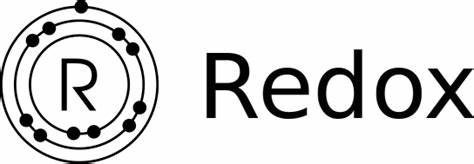
\includegraphics[width=1.\textwidth]{redox}
			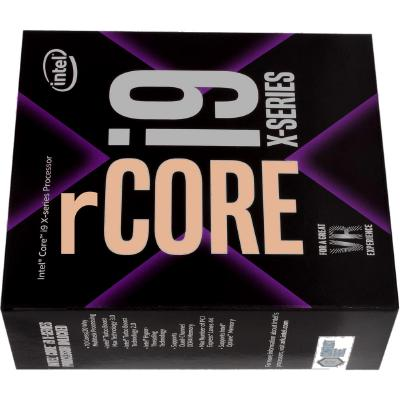
\includegraphics[width=1.\textwidth]{rcore}
			
\includegraphics[width=1.\textwidth]{firecracker}
		\end{column}
		
		\begin{column}{.8\textwidth}
			
						\Large
			
			Rust's central feature is ownership. 
			\begin{itemize}
			\item The Stack and the Heap
			\end{itemize}

			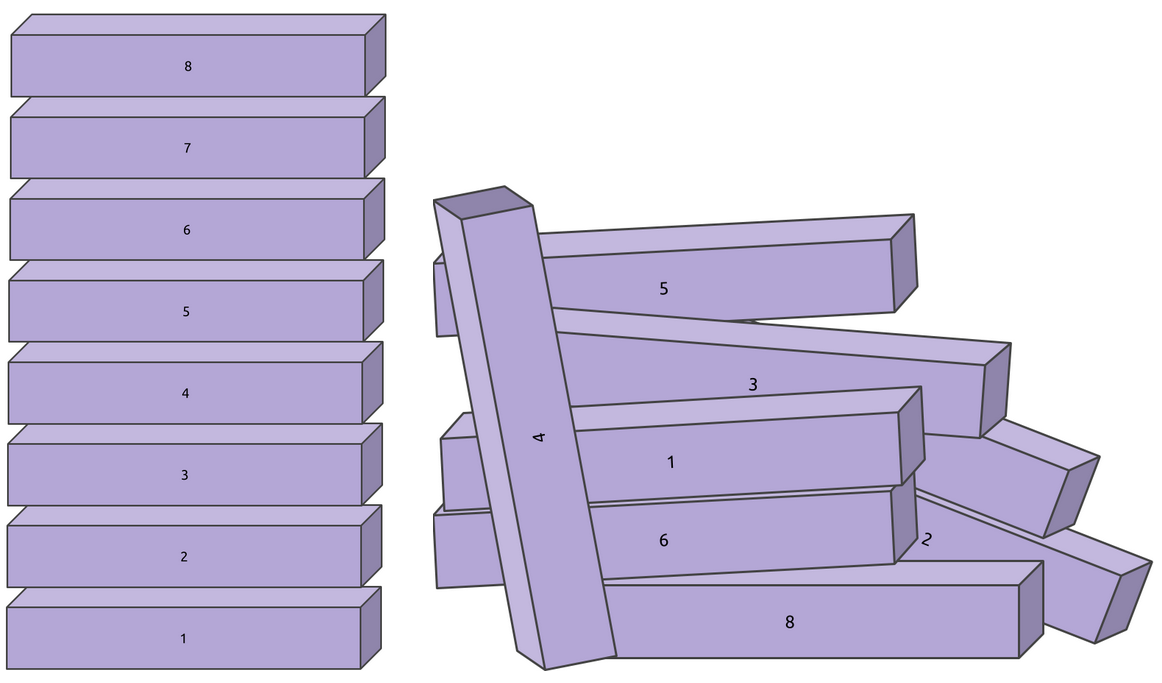
\includegraphics[width=.8\textwidth]{stack-heap}
		\end{column}
		
		
	\end{columns}
	
	
\end{frame}

%-------------------------------------------------
\begin{frame}[plain]
	\frametitle{Introduction -- OS in Rust -- Why Rust?}
	
	
	
	\begin{columns}
		
		\begin{column}{.4\textwidth}
			
			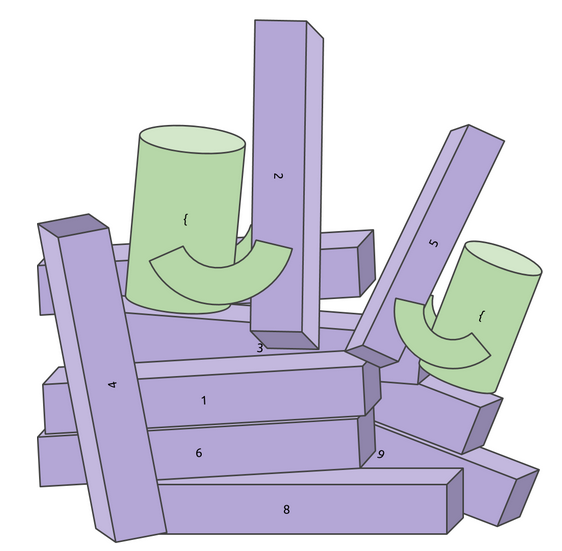
\includegraphics[width=1.\textwidth]{ownership}

		\end{column}
		
		\begin{column}{.6\textwidth}
			
			\Large
			
			Rust's central feature is ownership. 
			Keep these rules in mind :
			\begin{itemize}
				
				\item  Each value in Rust has a variable that’s called its owner.
				
				
				\item There can only be one owner at a time.
				
				\item When the owner goes out of scope, the value will be dropped.
				
				
			\end{itemize}
			
		\end{column}
		
		
	\end{columns}
	
	
\end{frame}


%-------------------------------------------------
\begin{frame}[plain]
	\frametitle{Introduction -- OS in Rust -- Why Rust?}
	
	
	
	\begin{columns}
		
		\begin{column}{.3\textwidth}
			
			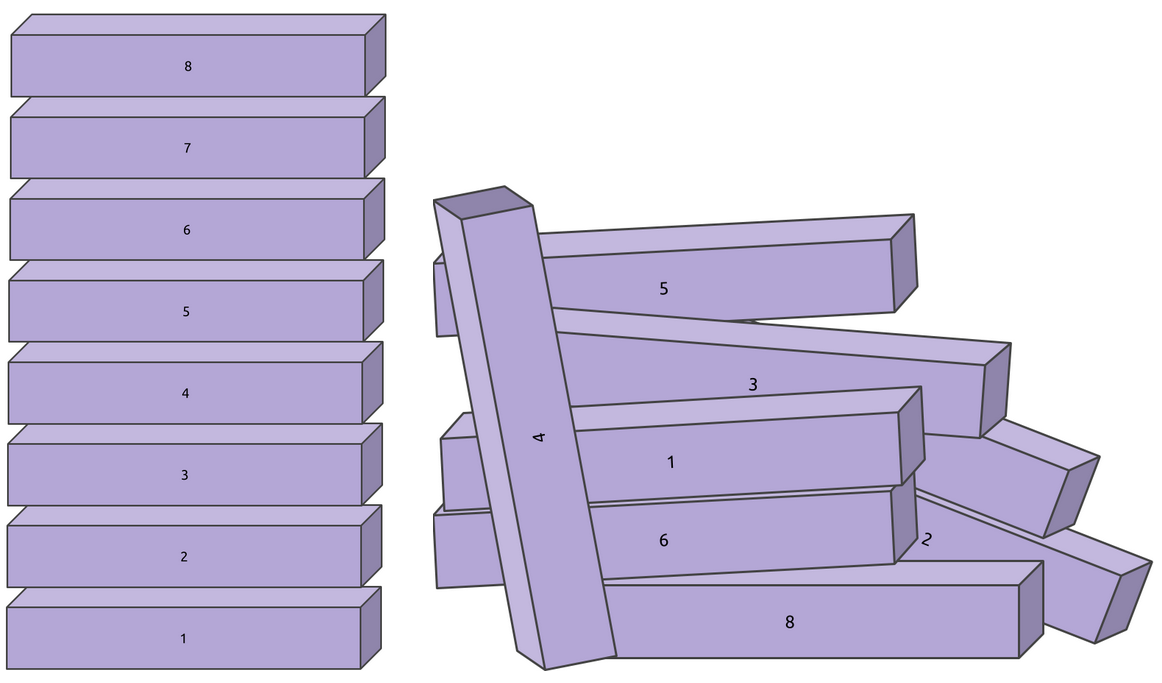
\includegraphics[width=1.\textwidth]{stack-heap}
			
		\end{column}
		
		\begin{column}{.7\textwidth}
			
			\Large
			
			Rust's central feature is ownership. 

			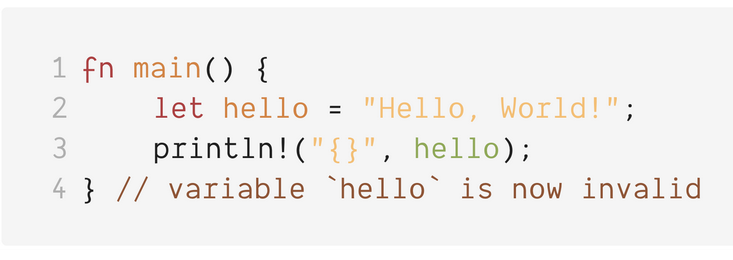
\includegraphics[width=1.\textwidth]{ownership-ex1}
			
		\end{column}
		
		
	\end{columns}
	
	
\end{frame}



%-------------------------------------------------
\begin{frame}[plain]
	\frametitle{Introduction -- OS in Rust -- Why Rust?}
	
	
	
	\begin{columns}
		
		\begin{column}{.3\textwidth}
			
			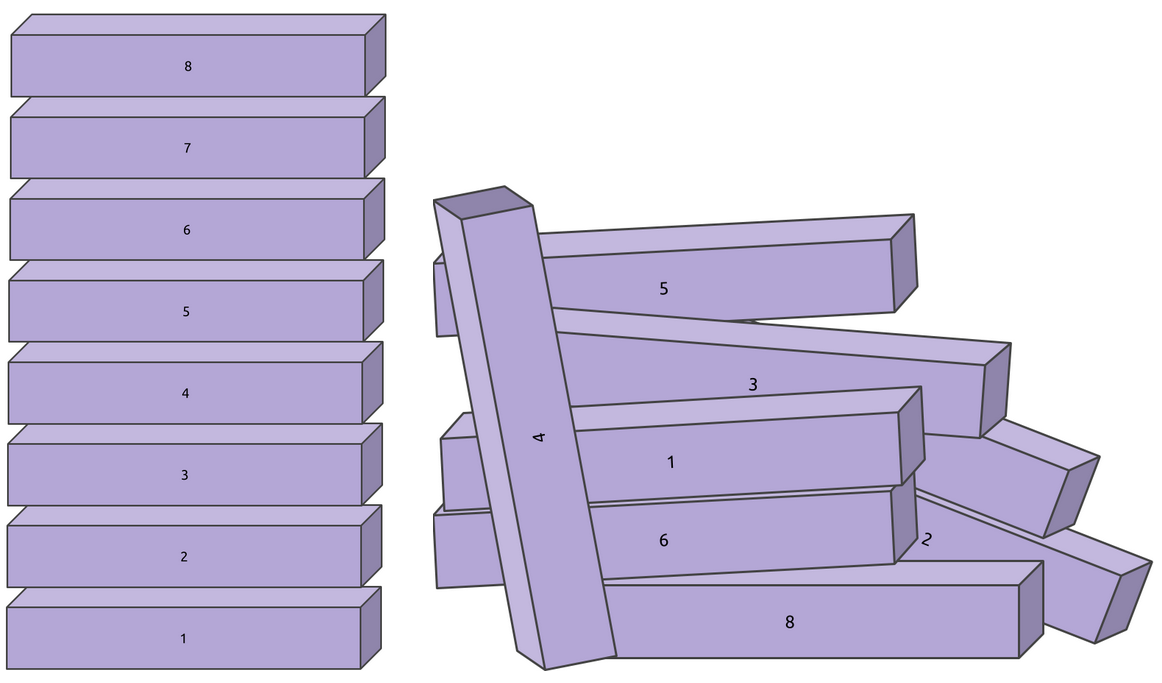
\includegraphics[width=1.\textwidth]{stack-heap}
			
		\end{column}
		
		\begin{column}{.7\textwidth}
			
			\Large
			
			Rust's central feature is ownership. 
			\\ 
			Copy vs Move
			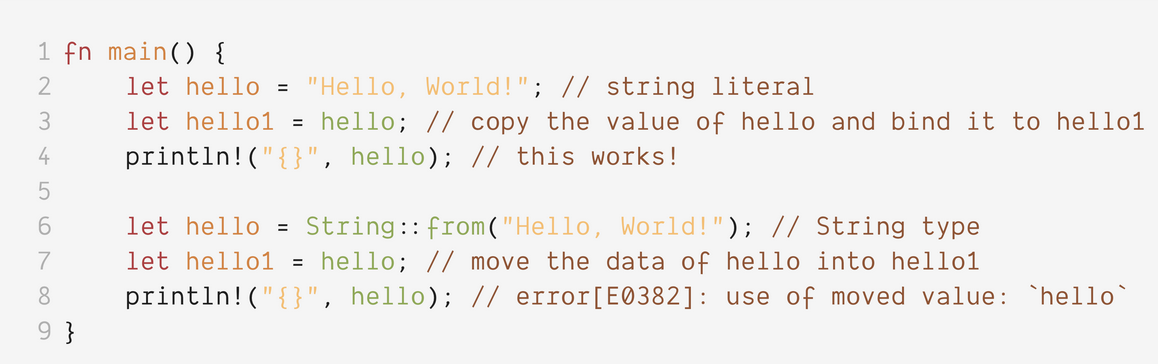
\includegraphics[width=1.\textwidth]{ownership-ex2}
			
		\end{column}
		
		
	\end{columns}
	
	
\end{frame}



%-------------------------------------------------
\begin{frame}[plain]
	\frametitle{Introduction -- OS in Rust -- Why Rust?}
	
	
	
	\begin{columns}
		
		\begin{column}{.5\textwidth}
			\Large
			Copy trait when using \&str 
			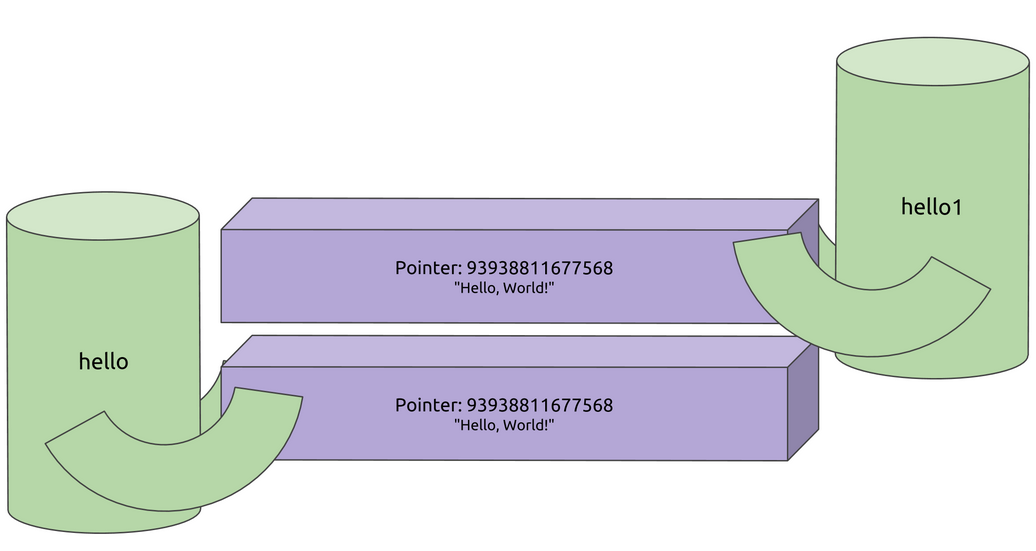
\includegraphics[width=1.\textwidth]{ownership-ex3}
			
		\end{column}
		
		\begin{column}{.5\textwidth}
			
			\Large
			

			Move trait when using the heap
			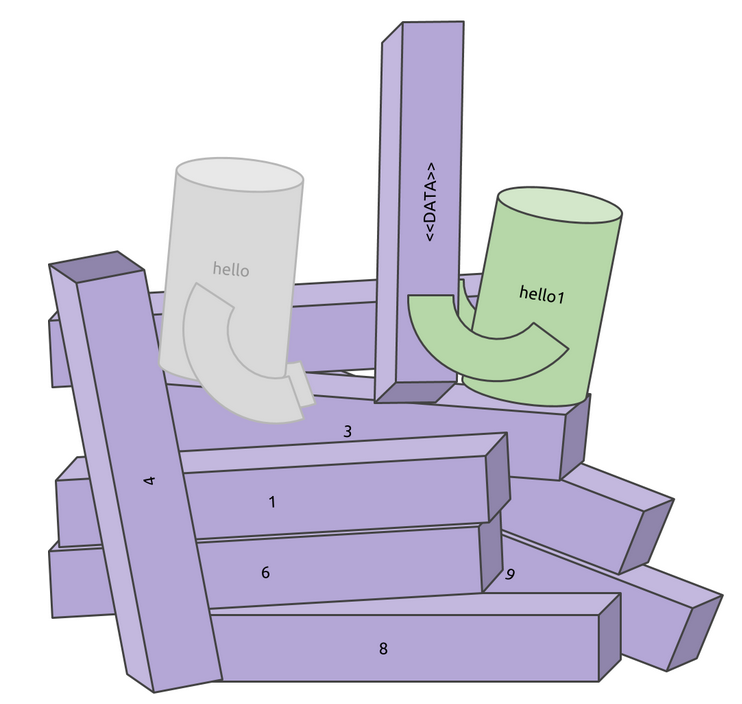
\includegraphics[width=1.\textwidth]{ownership-ex4}
			
		\end{column}
		
		
	\end{columns}
	
	
\end{frame}


%-------------------------------------------------
\begin{frame}[plain]
	\frametitle{Introduction -- OS in Rust -- Why Rust?}
	
	
	
	\begin{columns}
		
		\begin{column}{.5\textwidth}
			\Large
			A rough sketch of copying String type data 
			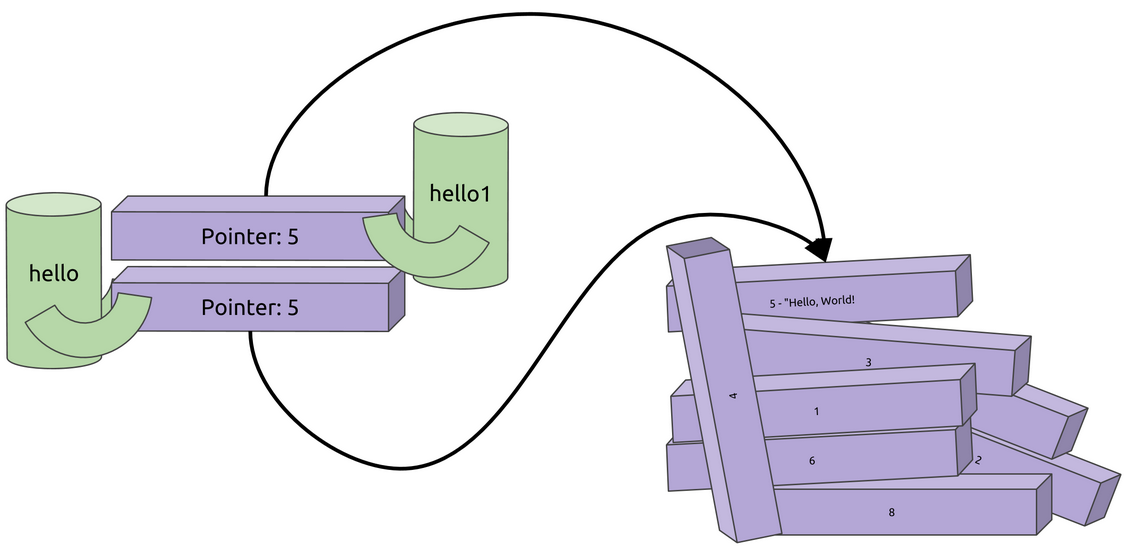
\includegraphics[width=1.\textwidth]{ownership-ex5}
			
		\end{column}
		
		\begin{column}{.5\textwidth}
			
			\Large
			
			
			Dropping hello1
			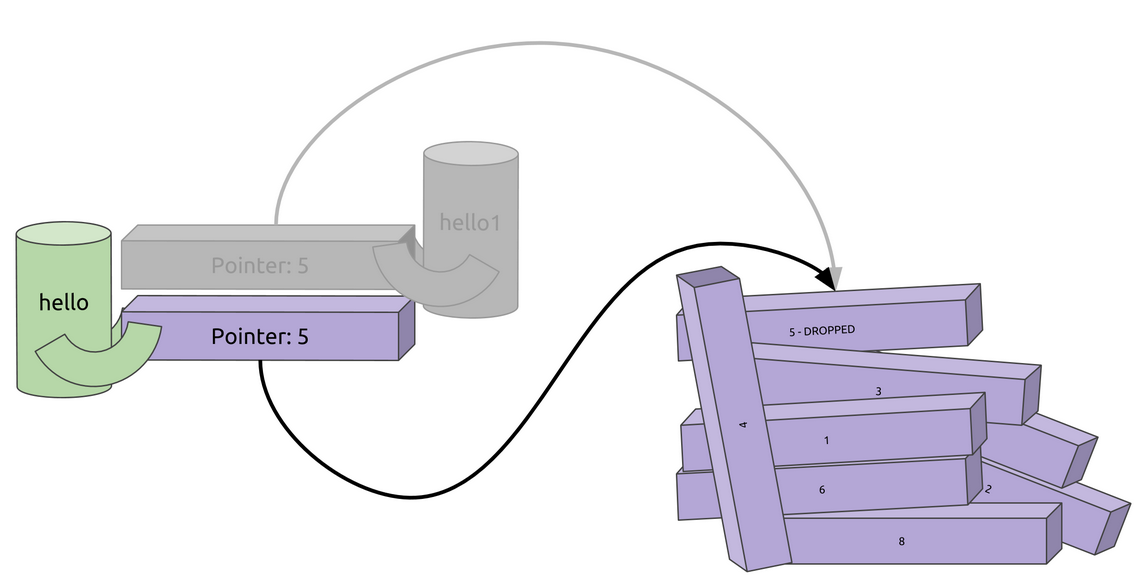
\includegraphics[width=1.\textwidth]{ownership-ex6}
			
		\end{column}
		
		
	\end{columns}
	
	
\end{frame}


%-------------------------------------------------
\begin{frame}[plain]
	\frametitle{Introduction -- OS in Rust -- Why Rust?}
	
	
	
	\begin{columns}
		
		\begin{column}{.3\textwidth}
			\Large
			Double Free Error
			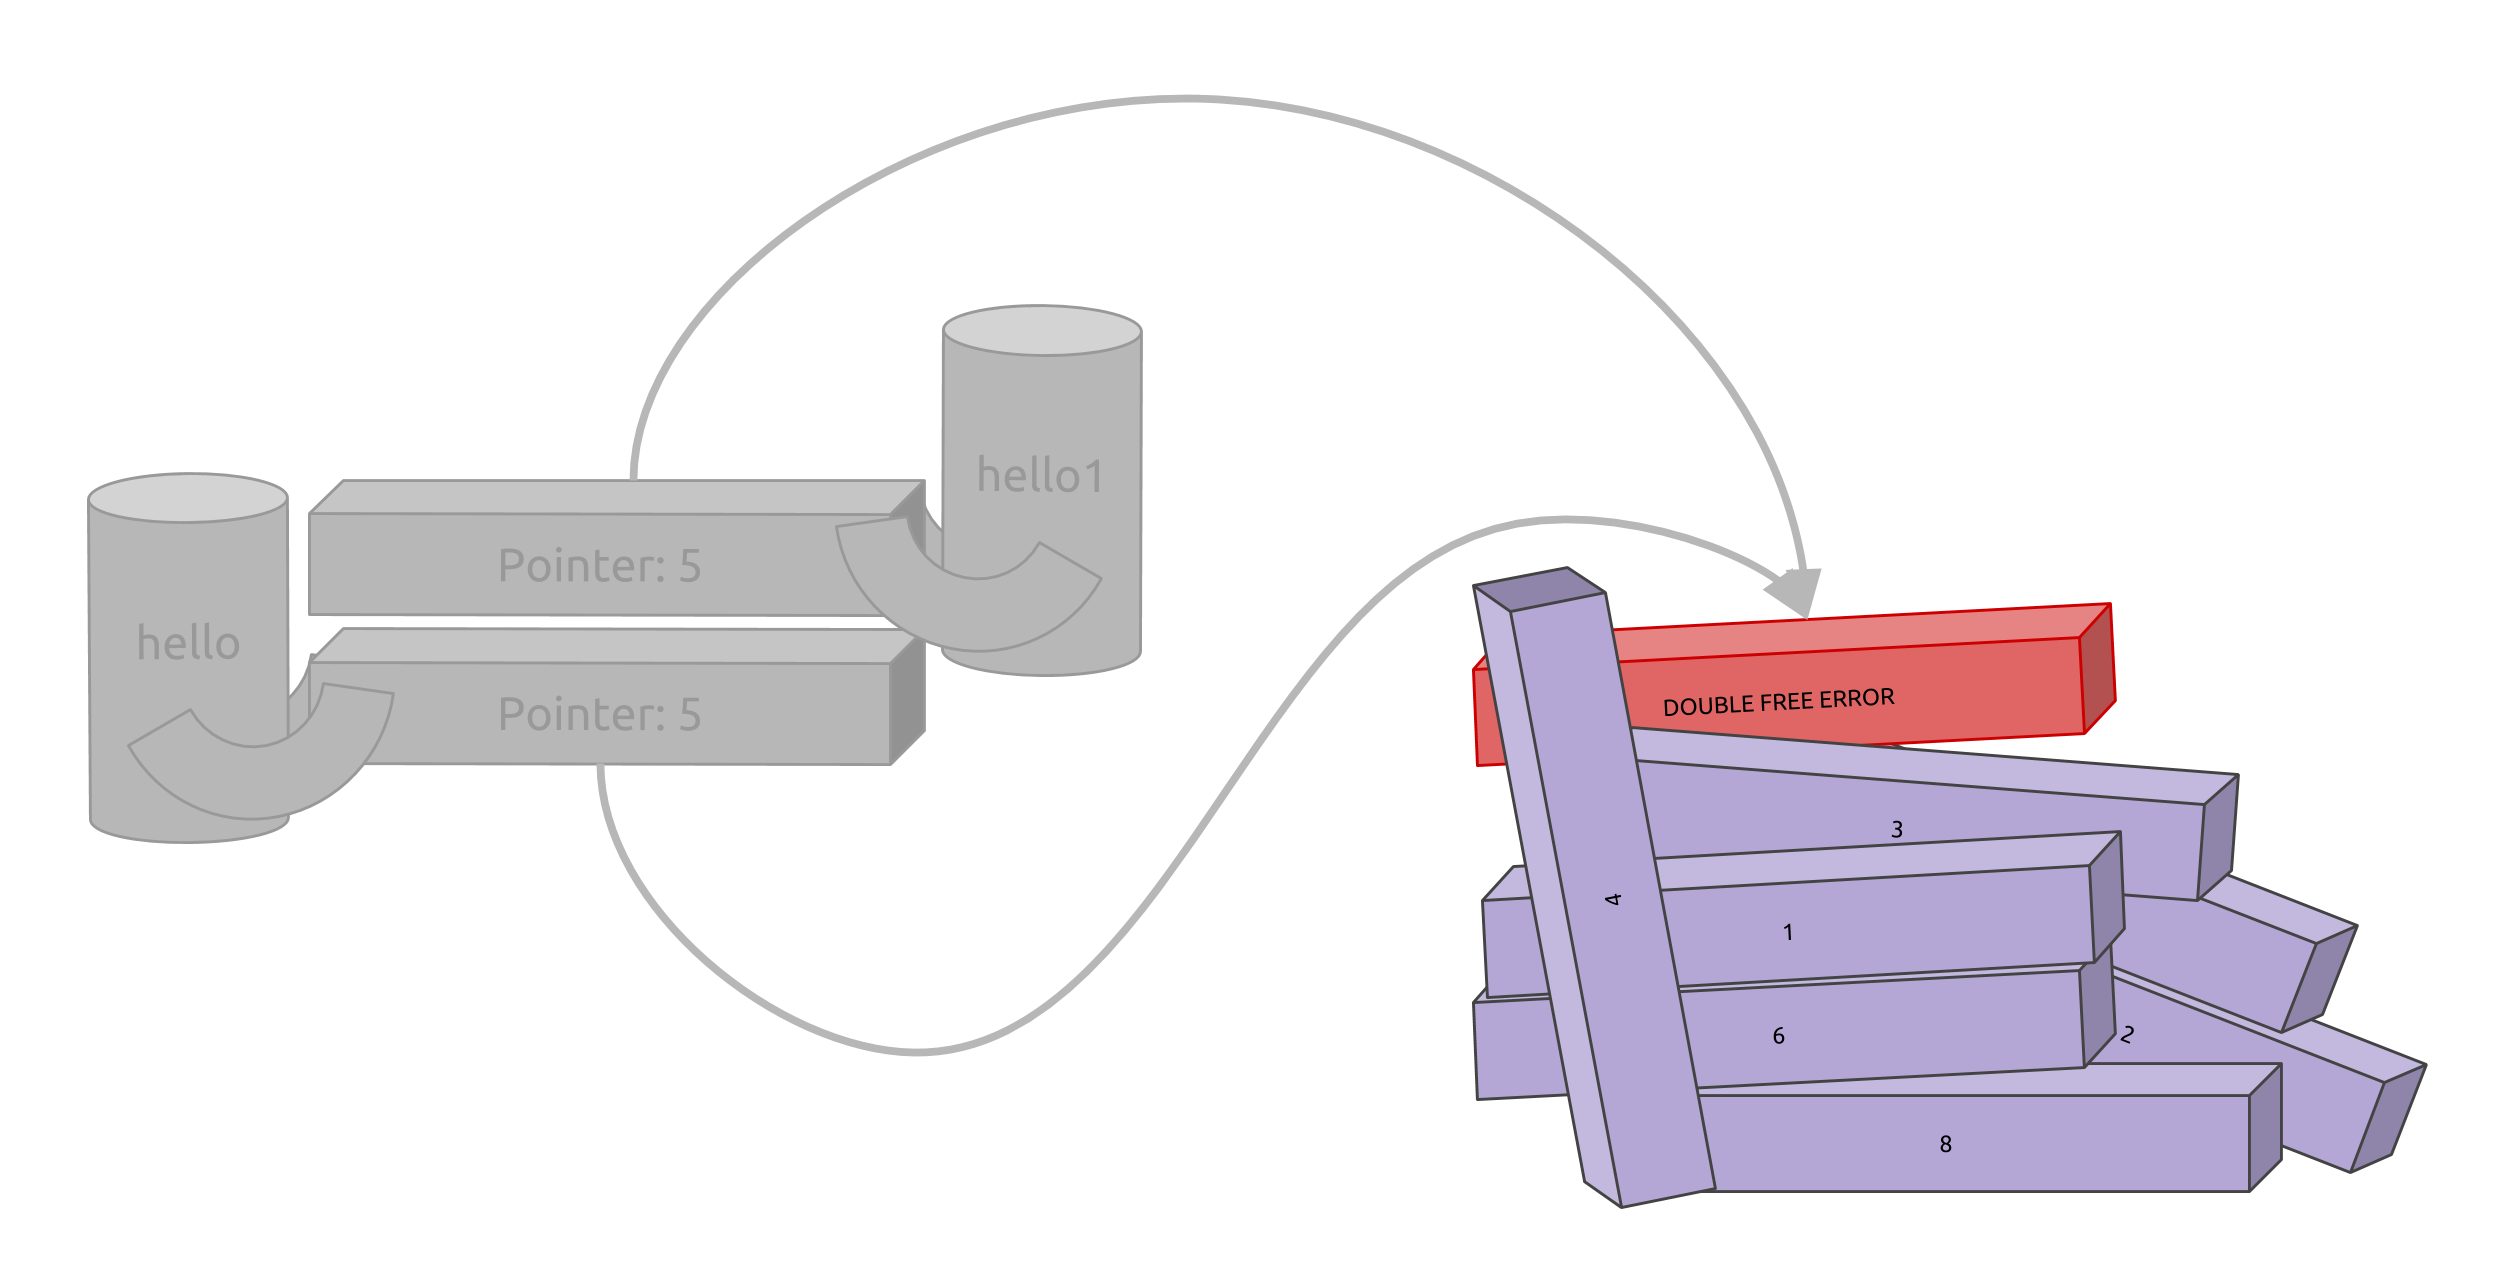
\includegraphics[width=1.\textwidth]{ownership-ex7}
			
		\end{column}
		
		\begin{column}{.7\textwidth}
			
			\Large
			
			
			Deep copy
			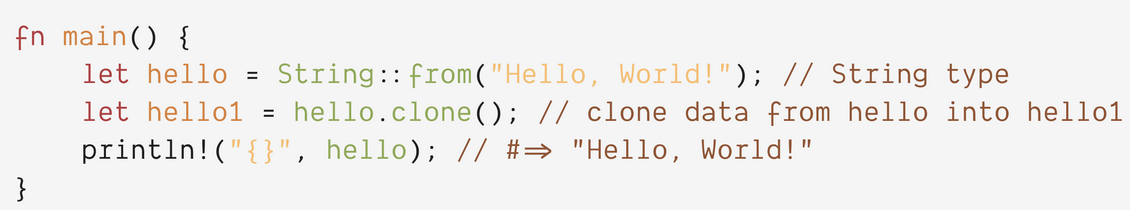
\includegraphics[width=1.\textwidth]{ownership-ex8}
			
		\end{column}
		
		
	\end{columns}
	
	
\end{frame}


%----------------------------------------------
\begin{frame}[plain]	
	\frametitle{Introduction -- OS in Rust -- Why Rust?}
	\centering
	\Large
	Ownership and Functions
	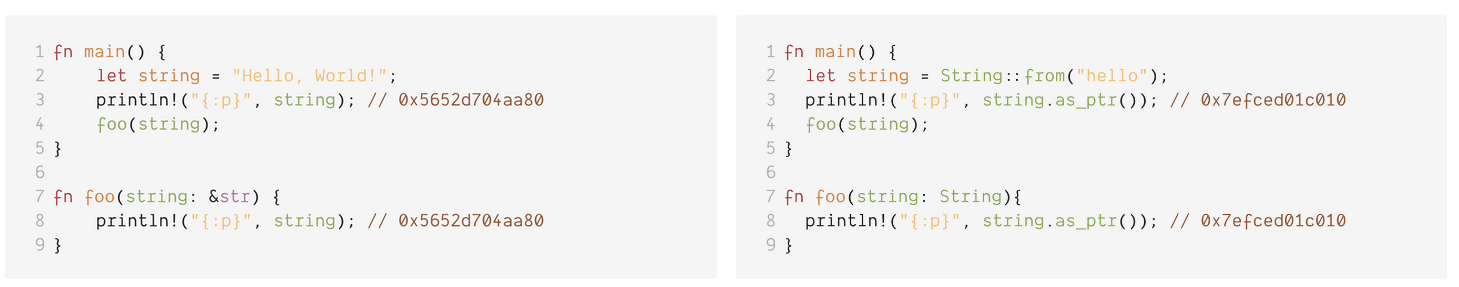
\includegraphics[width=1.\textwidth]{ownership-ex9}
	Copy versus Move
\end{frame}

%-------------------------------------------------
\begin{frame}[plain]
	\frametitle{Introduction -- OS in Rust -- Why Rust?}
	
	
	
	\begin{columns}
		
		\begin{column}{.5\textwidth}
			\centering
			\Large
			Copy
			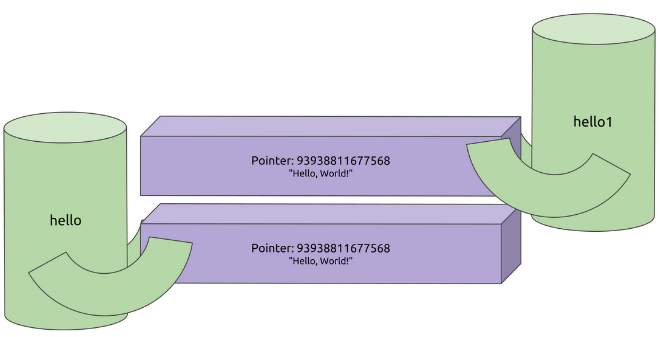
\includegraphics[width=1.\textwidth]{ownership-ex10}
			
		\end{column}
		
		\begin{column}{.5\textwidth}
			
			\Large
			
			
			Move
			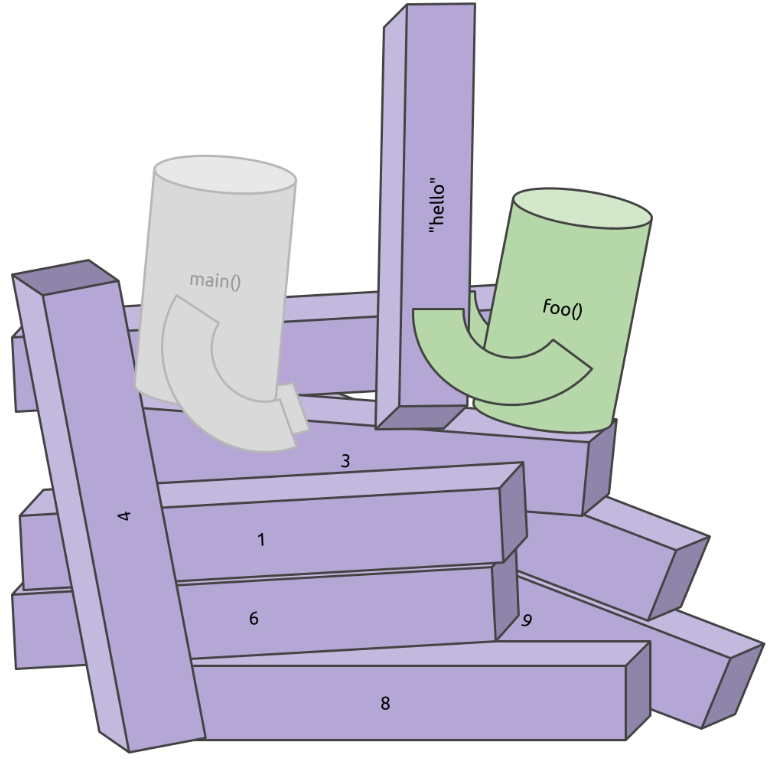
\includegraphics[width=.9\textwidth]{ownership-ex11}
			
		\end{column}
		
		
	\end{columns}
	
	
\end{frame}

%----------------------------------------------
\begin{frame}[plain]	
	\frametitle{Introduction -- OS in Rust -- Why Rust?}
	\centering
	\Large
	clone()
	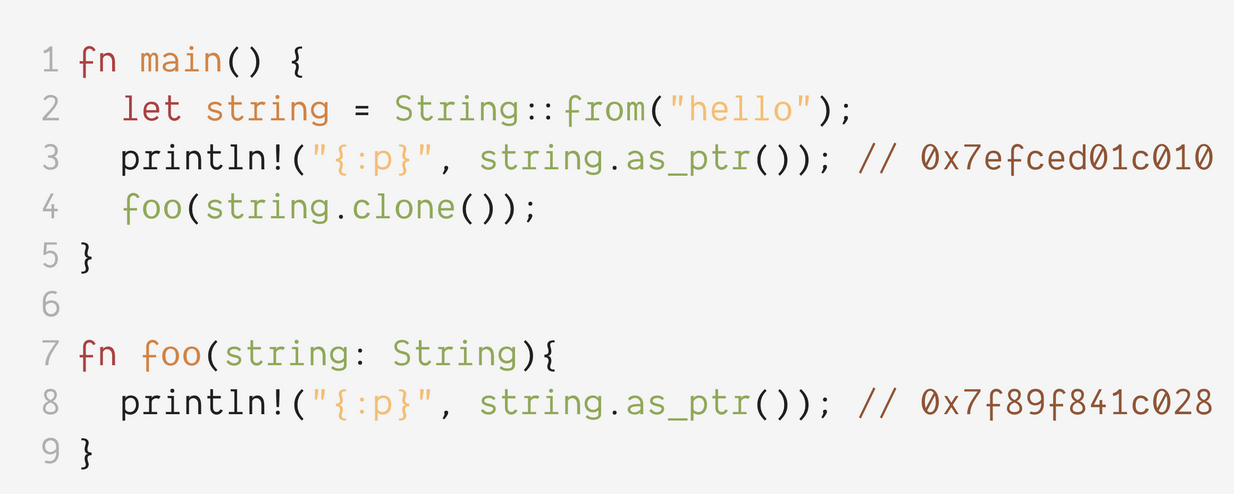
\includegraphics[width=.6\textwidth]{ownership-ex12}
	
	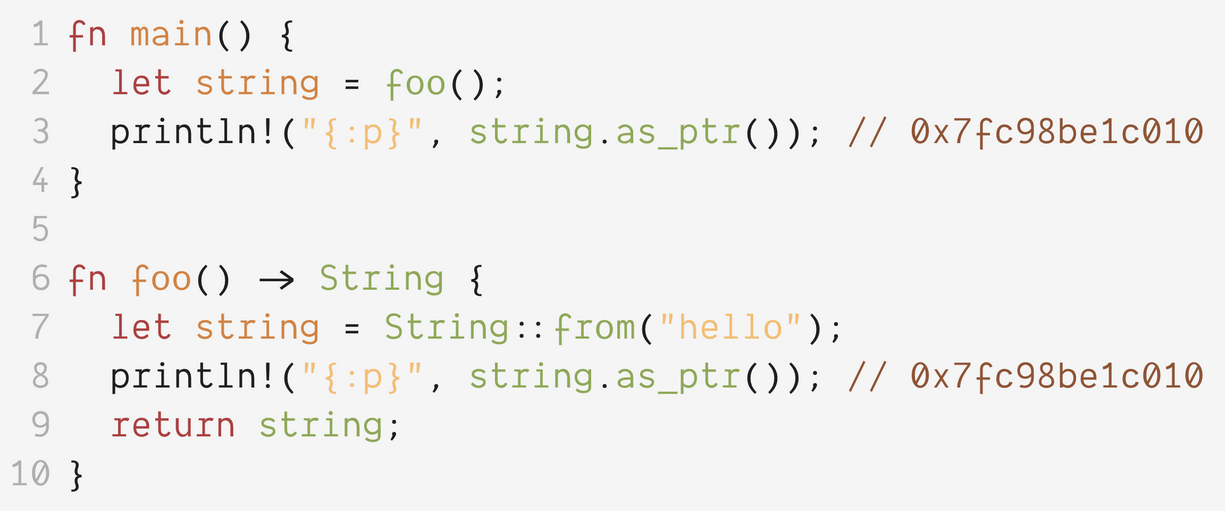
\includegraphics[width=.6\textwidth]{ownership-ex13}
	Giving ownership
\end{frame}



%-------------------------------------------------
\begin{frame}[plain]
	\frametitle{Introduction -- OS in Rust -- Why Rust?}
	
	
	
	\begin{columns}
		
		\begin{column}{.3\textwidth}
			\centering
			\Large
			borrowing
			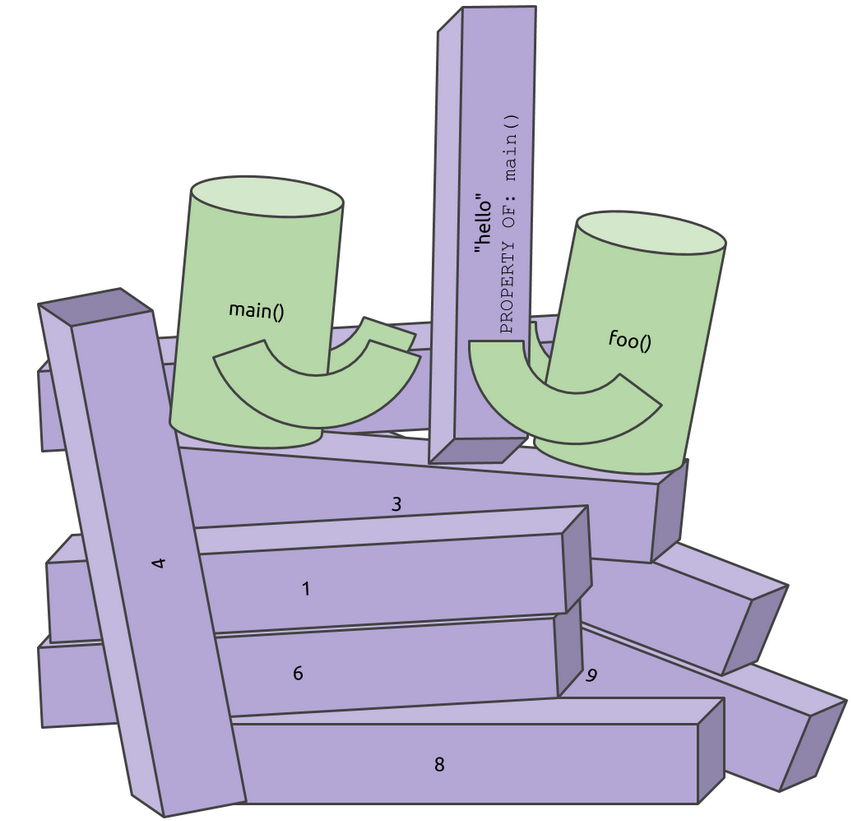
\includegraphics[width=1.\textwidth]{ownership-ex14}
			
		\end{column}
		
		\begin{column}{.7\textwidth}
			
			\Large
			
			
			Passing a reference/borrowing
			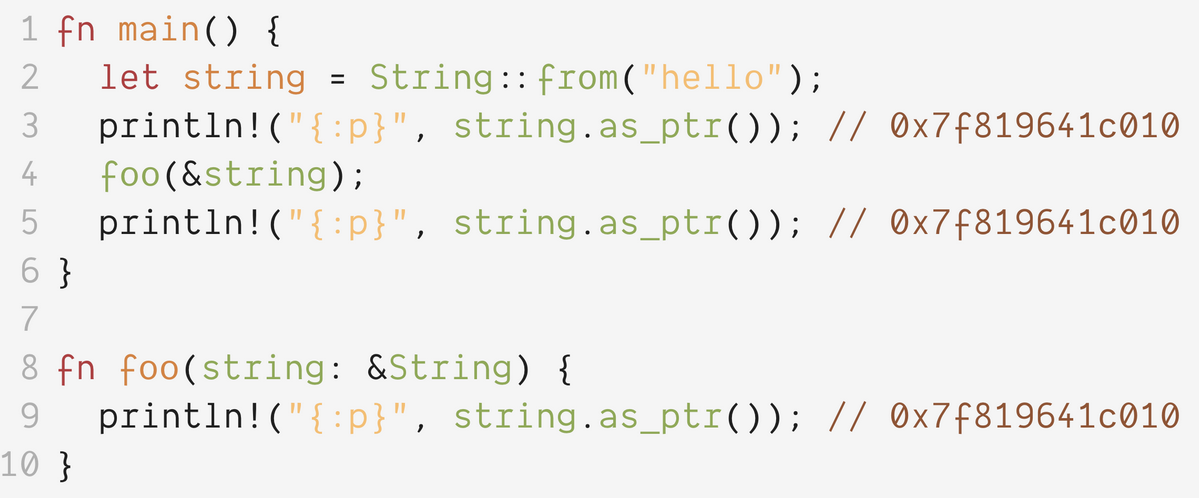
\includegraphics[width=1.\textwidth]{ownership-ex15}
			
		\end{column}
		
		
	\end{columns}
	
	
\end{frame}


%----------------------------------------------
\begin{frame}[plain]	
	\frametitle{Introduction -- OS in Rust -- Why Rust?}
	\centering
%	\Large
	Passing a mutable reference between functions
	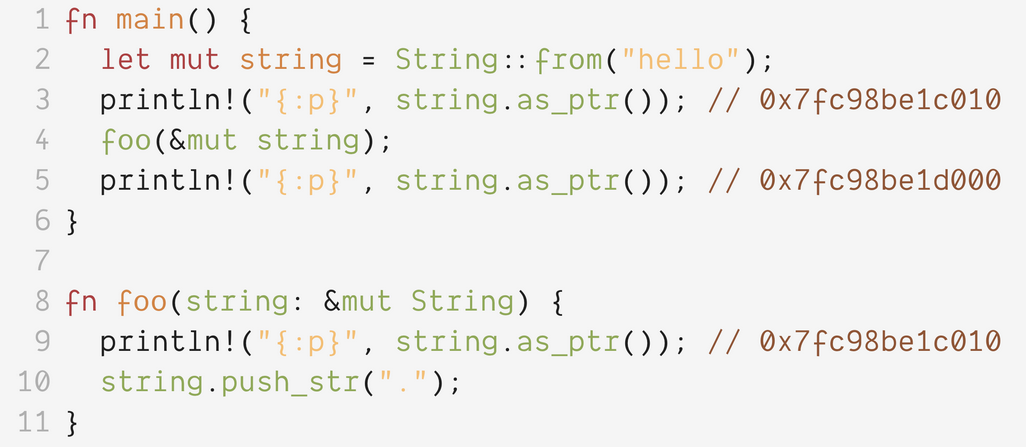
\includegraphics[width=.6\textwidth]{ownership-ex16}
	Dangling Reference, ERR!
	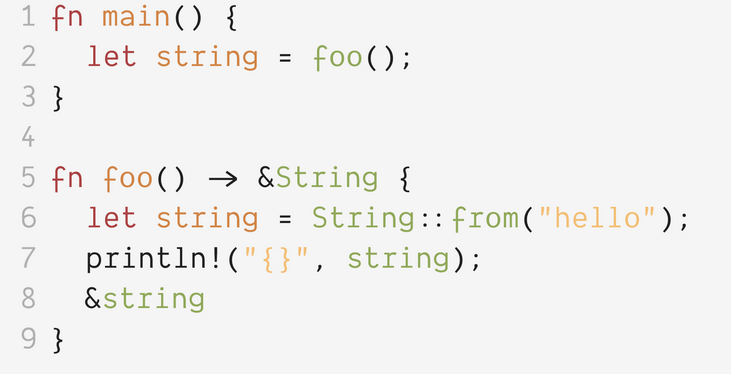
\includegraphics[width=.4\textwidth]{ownership-ex17}

\end{frame}
%-------------------------------------------------
\begin{frame}[plain]
	\frametitle{Introduction -- OS in Rust}
	
	
	
	\begin{columns}
		
		\begin{column}{.2\textwidth}
			
			
\includegraphics[width=1.\textwidth]{rust-logo}
			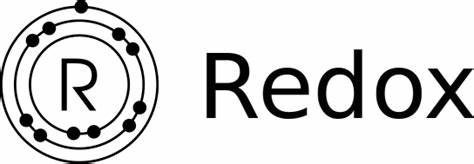
\includegraphics[width=1.\textwidth]{redox}
			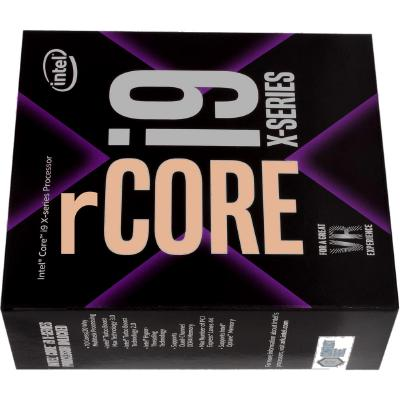
\includegraphics[width=1.\textwidth]{rcore}
			
\includegraphics[width=1.\textwidth]{firecracker}
		\end{column}
		
		\begin{column}{.8\textwidth}
			
%			\Large
		Is it time to rewrite the operating
		system in Rust?
		 \\
		
	Rust \&OS in the 2010s

\begin{itemize}
	
	\item  First attempt at an operating system kernel in Rust seems to be
	Alex Light’s Reenix, ca. 2015: a re-implementation of a teaching
	operating system in Rust as an undergrad thesis
	
	
	\item  Since Reenix’s first efforts, there have been quite a few small
	systems in Rust, e.g.: Redox, Tifflin, Tock, intermezzOS,
	RustOS/QuiltOS, Rux, and Philipp Oppermann’s Blog OS, and rcore.
	
	\item Some of these are teaching systems (intermezzOS, Blog OS),
	some are unikernels (QuiltOS) and/or targeted at IoT (Tock)
	
	
\end{itemize}

		\end{column}
		
		
	\end{columns}
	
	
\end{frame}

%-------------------------------------------------
\begin{frame}[plain]
	\frametitle{Introduction -- OS in Rust}
	
	
	
	\begin{columns}
		
		\begin{column}{.2\textwidth}
			
			
\includegraphics[width=1.\textwidth]{rust-logo}
			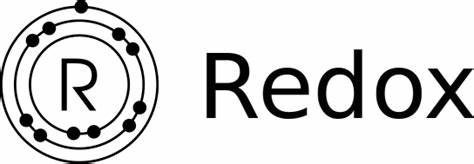
\includegraphics[width=1.\textwidth]{redox}
			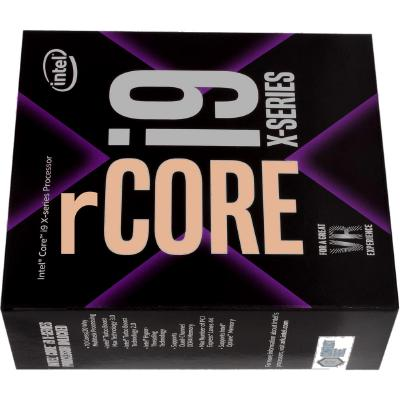
\includegraphics[width=1.\textwidth]{rcore}
			
\includegraphics[width=1.\textwidth]{firecracker}
		\end{column}
		
		\begin{column}{.8\textwidth}
			
			OS in Rust?
			
			\begin{itemize}
				
				\item  Rust is a systems software programming language designed
				around safety, parallelism, and speed
				
				\item Rust has a novel system of ownership, whereby it can statically
				determine when a memory object is no longer in use
				
				\item This allows for the power of a garbage-collected language, but
				with the performance of manual memory management
				
				\item  This is important because — unlike C — Rust is highly
				composable, allowing for more sophisticated (and higher
				performing!) primitives
				
				
			\end{itemize}
			
		\end{column}
		
		
	\end{columns}
	
	
\end{frame}

%----------------------------------------------
\begin{frame}[plain]	
	\frametitle{Introduction -- OS in Rust}
	\centering
	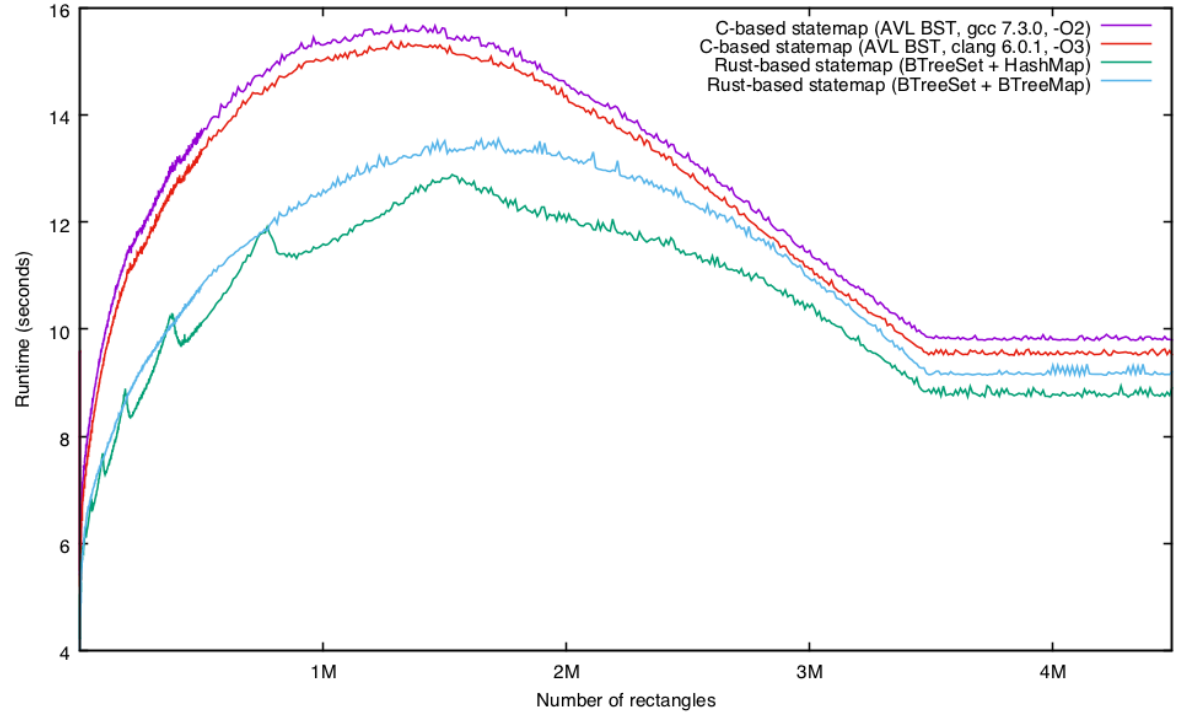
\includegraphics[width=.8\textwidth]{rust-perf}
	 \tiny Source: http://dtrace.org/blogs/bmc/2018/09/28/the-relative-performance-of-c-and-rust/
	 
\end{frame}



%-------------------------------------------------
\begin{frame}[plain]
	\frametitle{Introduction -- OS in Rust}
	
	
	
	\begin{columns}
		
		\begin{column}{.2\textwidth}
			
			
\includegraphics[width=1.\textwidth]{rust-logo}
			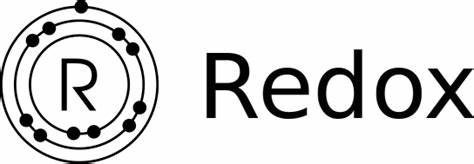
\includegraphics[width=1.\textwidth]{redox}
			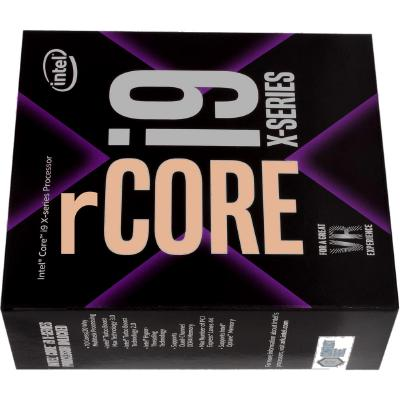
\includegraphics[width=1.\textwidth]{rcore}
			
\includegraphics[width=1.\textwidth]{firecracker}
		\end{column}
		
		\begin{column}{.8\textwidth}
			
			OS in Rust? \\
			Rust has a number of other features that make it highly
			compelling for systems software implementation:
			
			\begin{itemize}
				
				\item Algebraic types allow robust, concise error handling
				\item Hygienic macros allow for safe syntax extensions	
				\item Foreign function interface allows for full-duplex integration
				with C without sacrificing performance		
				\item  “unsafe” keyword allows for some safety guarantees to be
				surgically overruled (though with obvious peril)
				\item active community and ecosystem, etc.
				
				
				
			\end{itemize}
			
		\end{column}
		
		
	\end{columns}
	
	
\end{frame}


%-------------------------------------------------
\begin{frame}[plain]
	\frametitle{Introduction -- OS in Rust}
	
	
	
	\begin{columns}
		
		\begin{column}{.2\textwidth}
			
			
\includegraphics[width=1.\textwidth]{rust-logo}
			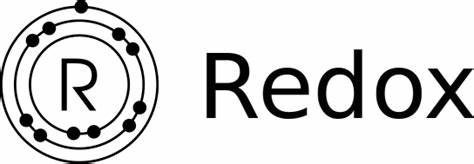
\includegraphics[width=1.\textwidth]{redox}
			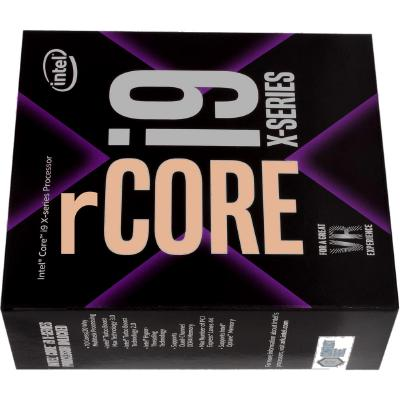
\includegraphics[width=1.\textwidth]{rcore}
			
\includegraphics[width=1.\textwidth]{firecracker}
		\end{column}
		
		\begin{column}{.8\textwidth}
			
			OS in Rust? \\
			Rust has a number of other features that make it highly
			compelling for systems software implementation:
			
			\begin{itemize}
				
				\item  If the history of operating systems implementation teaches us
				anything, it’s that runtime characteristics trump development
				challenges!
				
				\item  Structured languages (broadly) replaced assembly because
				they performed as well
				
				\item every operating system retains some assembly for reasons
				of performance!
						
				\item With its focus on performance and zero-cost abstractions, Rust
				does represent a real, new candidate programming language
				for operating systems implementation

			\end{itemize}
			
		\end{column}
		
		
	\end{columns}
	
	
\end{frame}



%-------------------------------------------------
\begin{frame}[plain]
	\frametitle{Introduction -- OS in Rust}
	
	
	
	\begin{columns}
		
		\begin{column}{.2\textwidth}
			
			
\includegraphics[width=1.\textwidth]{rust-logo}
			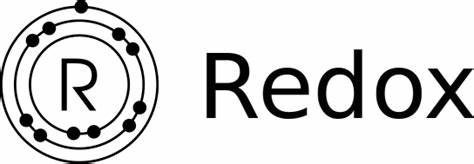
\includegraphics[width=1.\textwidth]{redox}
			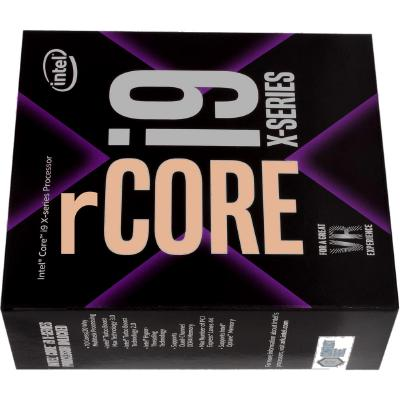
\includegraphics[width=1.\textwidth]{rcore}
			
\includegraphics[width=1.\textwidth]{firecracker}
		\end{column}
		
		\begin{column}{.8\textwidth}
			
			Challenges of OS in Rust? 
			
			\begin{itemize}
				
				\item While Rust’s advantages are themselves clear, it’s less clear
				what the advantage is when replacing otherwise working code
				
				\item   For in-kernel code in particular, the safety argument for Rust carries less weight: in-kernel C tends to be de facto safe

				\item Rust does, however, presents new challenges for kernel
				development, esp. with respect to multiply-owned structures

				\item An OS kernel - despite its historic appeal and superficial fit for	Rust - may represent more challenge than its worth
				
				
			\end{itemize}
			But what of hybrid/other approaches?
			
		\end{column}
		
		
	\end{columns}
	
	
\end{frame}


%-------------------------------------------------
\begin{frame}[plain]
	\frametitle{Introduction -- OS in Rust}
	
	
	
	\begin{columns}
		
		\begin{column}{.2\textwidth}
			
			
\includegraphics[width=1.\textwidth]{rust-logo}
			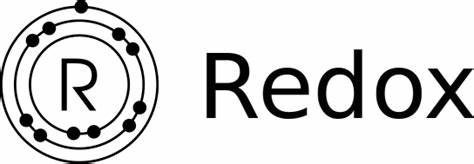
\includegraphics[width=1.\textwidth]{redox}
			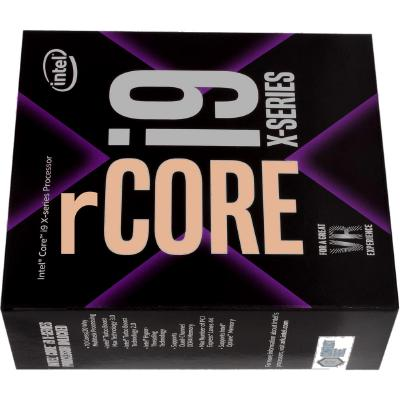
\includegraphics[width=1.\textwidth]{rcore}
			\includegraphics[width=1.\textwidth]{firecracker}
		\end{column}
		
		\begin{column}{.8\textwidth}
			
			OS in Rust? \\
			Rust has a number of other features that make it highly
			compelling for systems software implementation:
			
			\begin{itemize}
				
				\item  If the history of operating systems implementation teaches us
				anything, it’s that runtime characteristics trump development
				challenges!
				
				\item  Structured languages (broadly) replaced assembly because
				they performed as well
				
				\item every operating system retains some assembly for reasons
				of performance!
				
				\item With its focus on performance and zero-cost abstractions, Rust
				does represent a real, new candidate programming language
				for operating systems implementation
				
			\end{itemize}
			
		\end{column}
		
		
	\end{columns}
	
	
\end{frame}



%-------------------------------------------------
\begin{frame}[plain]
	\frametitle{Introduction -- OS in Rust}
	
	
	
	\begin{columns}
		
		\begin{column}{.2\textwidth}
			
			\includegraphics[width=1.\textwidth]{rust-logo}
			\includegraphics[width=1.\textwidth]{redox}
			\includegraphics[width=1.\textwidth]{rcore}
			\includegraphics[width=1.\textwidth]{firecracker}
		\end{column}
		
		\begin{column}{.8\textwidth}
			
			Hybrid approach I: Rust in-kernel components
			
			
			\begin{itemize}
				
				\item One appeal of Rust is its ability to interoperate with C
				
				
				\item One hybrid approach to explore would be to retain a
				C-/assembly-based kernel while allowing for Rust-based
				in-kernel components like device drivers and filesystems
				
				\item  This would allow for an incremental approach — and instead of
				rewriting, Rust can be used for new development
				
				
				\item An There is a prototype example of this in FreeBSD/Linux; others are	presumably possible
				
				
				
			\end{itemize}
			
		\end{column}
		
		
	\end{columns}
	
	
\end{frame}


%-------------------------------------------------
\begin{frame}[plain]
	\frametitle{Introduction -- OS in Rust}
	
	
	
	\begin{columns}
		
		\begin{column}{.2\textwidth}
			
			\includegraphics[width=1.\textwidth]{rust-logo}
			\includegraphics[width=1.\textwidth]{redox}
			\includegraphics[width=1.\textwidth]{rcore}
			\includegraphics[width=1.\textwidth]{firecracker}
		\end{column}
		
		\begin{column}{.8\textwidth}
			
			Hybrid approach II: Rust OS components

			\begin{itemize}
				
				\item  An operating system is not just a kernel!

				\item Operating systems have significant functionality at user-level:
				utilities, daemons, service-/device-/fault- management facilities,
				debuggers, etc.

				\item  If anything, the definition of the OS is expanding to distributed
				system that represents a multi-computer control plane — that
				itself includes many components
				
				
				\item These components are much more prone to run-time failure.
				
				\item Many of these are an excellent candidate for Rust.
				
			\end{itemize}
			
		\end{column}
		
		
	\end{columns}
	
	
\end{frame}


%-------------------------------------------------
\begin{frame}[plain]
	\frametitle{Introduction -- OS in Rust}
	
	
	
	\begin{columns}
		
		\begin{column}{.2\textwidth}
			
			\includegraphics[width=1.\textwidth]{rust-logo}
			\includegraphics[width=1.\textwidth]{redox}
			\includegraphics[width=1.\textwidth]{rcore}
			\includegraphics[width=1.\textwidth]{firecracker}
		\end{column}
		
		\begin{column}{.8\textwidth}
			
			Hybrid approach III: Rust-based firmware/hypervisor

			\begin{itemize}
				
				\item  Below the operating system lurks hardware-facing special-
				purpose software: firmware/hypervisor
				
				
				\item Firmware/hypervisor is a sewer of unobservable software with a long
				history of infamous quality problems
				
				
				\item  Firmware has some of the same challenges as kernel
				development (e.g., dealing with allocation failures), but may
				otherwise be more amenable to Rust

				\item This is especially true when/where firmware is in user-space
				and is network-facing! (e.g., OpenBMC/OpenSBI)
				
			\end{itemize}
			
		\end{column}
		
		
	\end{columns}
	
	
\end{frame}

%-------------------------------------------------
\begin{frame}[plain]
	\frametitle{References}
	
	\begin{itemize}
		
		\item Is it time to rewrite the operating system in Rust? Bryan Cantrill, tech talk, 2018
		\item Ownership in Rust, Thomas Countz, 2018
		
		
		
	\end{itemize}
	
	
\end{frame}
%-------------------------------------------------
%-------------------------------------------------
\end{document}